\documentclass[oneside,a4paper,12pt]{article}
\usepackage{graphicx}
\usepackage{amsmath}
\usepackage{listings}
\graphicspath{{~/templates/}, {../images/}}

\makeindex
\begin{document}
	\begin{titlepage}
		\includegraphics[width=4cm]{logopopo.png}
		\hspace*{\fill}
		\includegraphics[width=6cm]{logouniv.png}
		
		\begin{center}
			\vspace{1cm}
			\textbf{TP Support de Transmission}\\
			\textbf{Mélageur à diode}\\
			\vspace{1cm}
			\textbf{Maxence LAURENT, Thibault VOLLERIN, Maxence NEUS}\\
			\vspace{3cm}
			%\includegraphics[width=13cm]{titlepage.png}\\
			\vspace{\fill}
			\textbf{Mars 2022}\\
		\end{center}
	\end{titlepage}
	
	\tableofcontents
	
	\vspace{5cm}
	
	\begin{abstract}
	Le but de ce TP est de caractèriser un mélangeur à diode simple. Pour ce la on dispose d'un générateur
	2.5 GHz qui fera office de voie RF et d'un oscillateur programable qui nous servira de voie OL.
	Nous allons tracer les caractèristiques du mélangeur en fonction de la fréquence RF et OL pour les comparer à la datasheet.
 	\end{abstract}

	\newpage

	\section{Préparation}
	
	\paragraph{1.}
	 On donne le schéma équivalent du mélangeur à diode:
	 \begin{figure}[h]
		 \centering
		 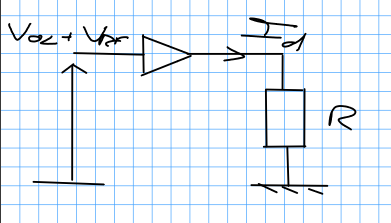
\includegraphics[width=8cm]{fig1.png}
		 \caption{Schéma équivalent du mélangeur à diode}
	 \end{figure}

	Si on néglige la chute de tension aux bornes de la résistance, on a:
	\[ I_{d}=I_{s}(e{q\frac{V_{OL}+V_{RF}}{kT}} -1) \]

	En linéarisant l'équation, on obtient:
	\[ I_{d} = a_{0} + a_{1}(V_{OL} + V_{RF}) + a_{2}(V_{OL} + V_{RF})^{2} + a_{3}(V_{OL} + V_{RF})^{3} + \cdots \]

	\paragraph{2.}
	Supposont $ V_{RF} = |V_{RF}|sin(2 \pi f_{RF}) $ et $ V_{OL} = |V_{OL}|sin(2 \pi f_{OL}) $

	On détermine les fréquences associées à chaqun des termes de $I_{d}$:

	\paragraph{A l'ordre 1:} 
	On a simplement $V_{OL} + V_{RF}$, on a donc une raie à $f_{OL}$ et une à $f_{RF}$.
	
	\paragraph{A l'ordre 2:}

	On a:
	\[ (V_{OL} + V_{RF})^{2} = V_{OL}^{2} + 2V_{OL}V_{RF} + V_{RF}^{2} \]

	\[ V_{OL}^{2} = \frac{|V_{OL}|^{2}}{2} sin(2 \pi 2 f_{OL}) \]
	Ce qui donne une raie à $2f_{OL}$.\\
	On a le même calcul pour $V_{RF}^{2}$ qui donne une raie à $2f_{RF}$.

	\[ 2 V_{OL} V_{RF} = |V_{OL}||V_{RF}|(cos(2 \pi (f_{OL} - f_{RF})) - cos(2 \pi (f_{OL} + f_{RF}))) \]
	 Soit une raie à $f_{OL}-f_{RF}$ et une à $f_{OL}+f_{RF}$

	\paragraph{A l'ordre 3:}
	On a:
	\[ (V_{OL} + V_{RF})^{3} = V_{OL}^{3} + 3V_{OL}^{2}V_{RF} + 3V_{OL}V_{RF}^{2} + V_{RF}^{3} \]
	\[ V_{OL}^{3} = \frac{|V_{OL}|^{3}}{2} ( sin(2 \pi f_{OL}) - cos(2 \pi 2 f_{OL}) sin(2 \pi f_{OL}) ) \]
	or \[ cos(2 \pi 2 f_{OL}) sin(2 \pi f_{OL}) = \frac{1}{2} ( sin(2 \pi 3 f_{OL}) - sin(2 \pi f_{OL}) ) \]
	Soit une raie à $3 f_{OL}$.
	On trouve de même une raie à $3 f_{RF}$.

	\[ 3 V_{OL}^{2} * V_{RF} = \frac{3 |V_{OL}|^{2} |V_{RF}|}{2} (sin(2 \pi f_{RF}) - cos(2 \pi 2 f_{OL}) sin(2 \pi f_{RF}) ) \]
	\[ cos(2 \pi 2 f_{OL}) sin(2 \pi f_{RF}) = \frac{1}{2} (sin(2 \pi ( 2 f_{OL} + f_{RF})) - sin(2 \pi (2 f_{OL} + f_{RF})) ) \]
	On a donc deux raies à $2 f_{OL} + f_{RF}$ et $2 f_{OL} - f_{RF}$.

	De même pour le terme $3 V_{OL} * V_{RF}^{2}$ on obtient deux raies à $ 2 f_{RF} + f_{OL} $ et  $ 2 f_{RF} - f_{OL} $.

	Pour une utilisation en down converter, la raie qui nous intéresse est cele à $ f_{OL} + f_{RF} $ à l'ordre 2.

	\newpage

	\section{Manipulations}

	\subsection{Etalonage}

	Il est nécessaire de calibrer les atténuateurs pour connaître la puissance injectée au mélangeur.
	Pour cela on fait varier la valeur de l'atténuateur pour avoir une puissance prédéfini à l'entrée du mélangeur.
	
	\subsection{Isolations}

	On visualise le spectre de puissance en voie IF autour des fréquences $f_{RF}$ et $f_{OL}$:

	\begin{figure}[h]
		\centering
		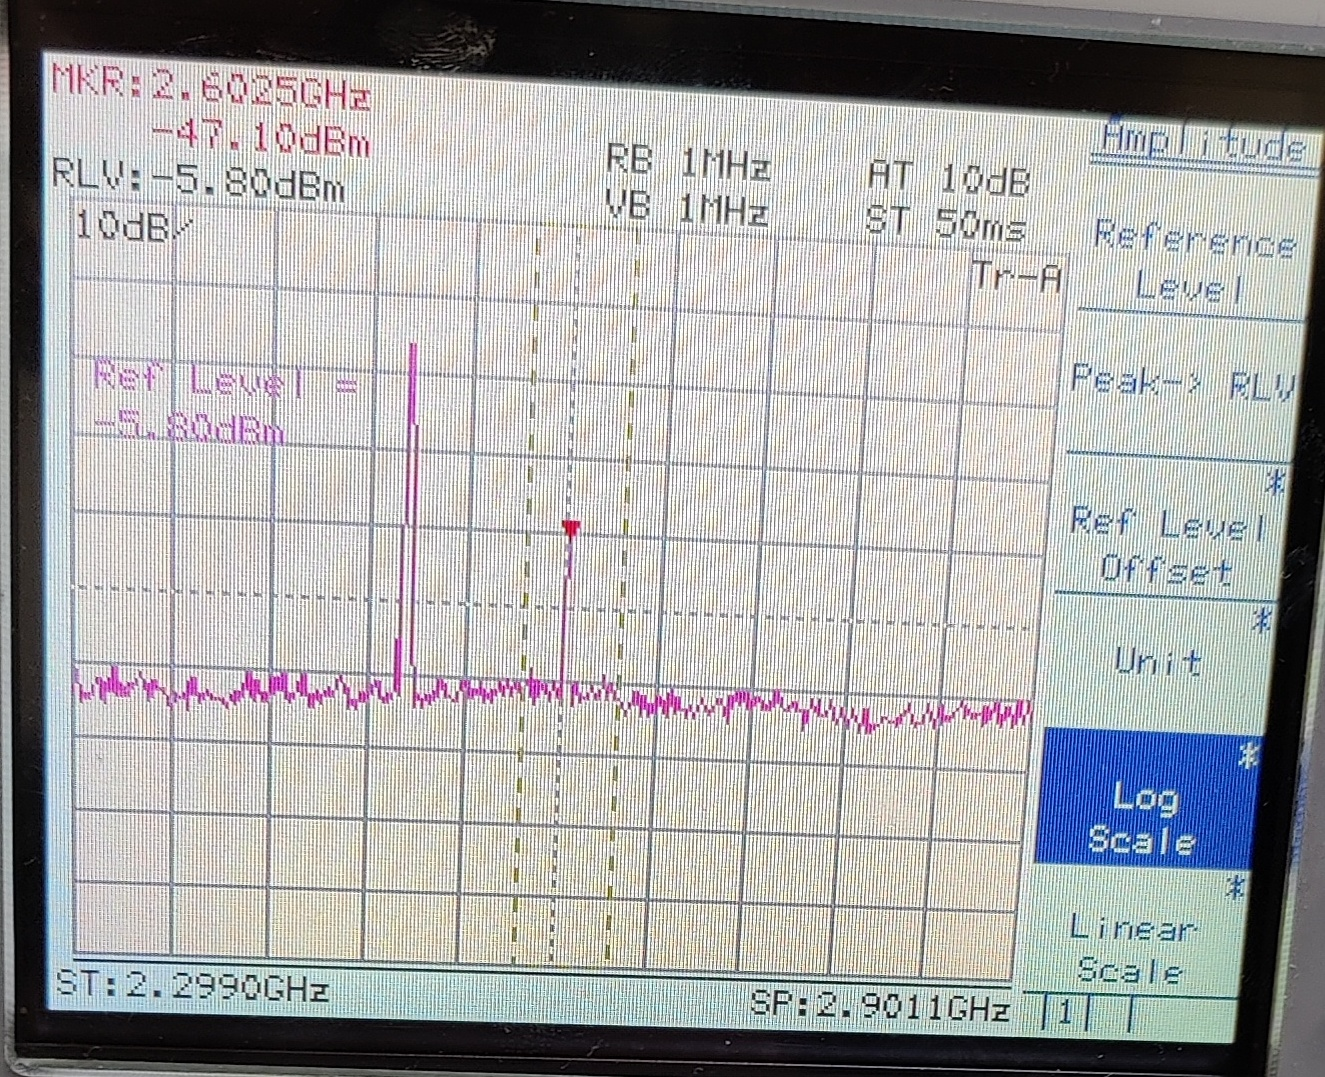
\includegraphics[width=8cm]{manip1.jpg}	
		\caption{Raies en voie IF}
	\end{figure}

	On a mesuré les puissances des raies :
	\[ P_{OL}(IF) = -22dBm \]
	\[ P_{RF}(IF) = -47dBm \]

	On en déduit les isolations:
	\[ I_{RF_IF} = P_{RF}(RF) - P_{RF}(IF) = (-20 dBm) - (-47 dBm) \]
	\[ I_{RF_IF} = 27 dB \]

	\[ I_{OL_IF} = P_{OL}(OL) - P_{OL}(IF) = (7 dBm) - (-22 dBm) \]
	\[ I_{OL_IF} = 29 dB \]

	\newpage

	\subsection{Pertes de conversion}

	On a mesuré la puissance à $f = f_{RF}-f_{OL}$ pour déterminer les pertes de convertion :
	\[ P_{RF}(RF) - P_{RF-OL}(IF)  \]

	\begin{figure}[h]
		\centering
		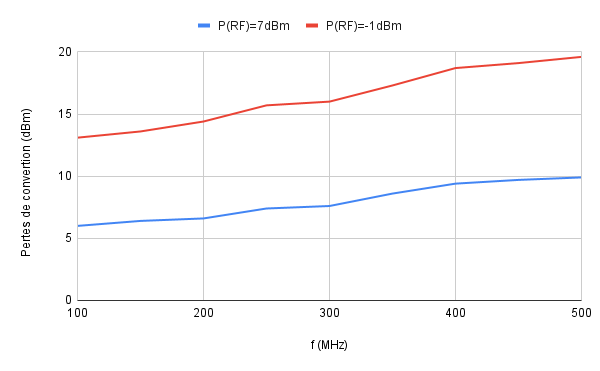
\includegraphics[width=10cm]{pertesfIF.png}	
		\caption{Pertes de convertions en fonction de $f_{IF}$}
	\end{figure}

	On voit que comme indiqué sur la datasheet, les pertes en convertion sont constantes pour $f_{RF}$ à 200MHz autour de $f_{OL}$.
	
	\begin{figure}[h]
		\centering
		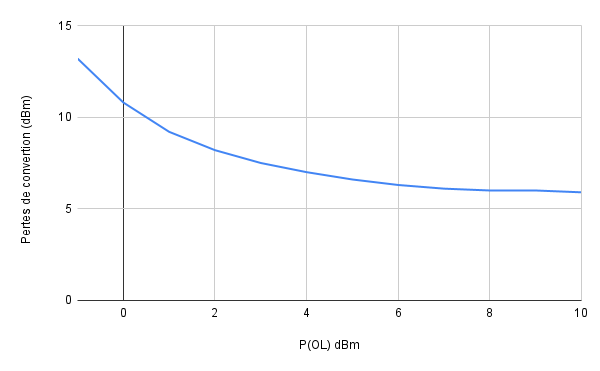
\includegraphics[width=10cm]{manip2.png}	
		\caption{Pertes de convertions en fonction de $P_{OL}$}
	\end{figure}

	On observe que les pertes de convertion décroissent quand $P_{OL}$ augmente, en effet plus $P_{OL}$ est grand,
	plus le mélangeur oppère dans une plage non linéaire et est donc plus efficace.

	\begin{figure}[h]
		\centering
		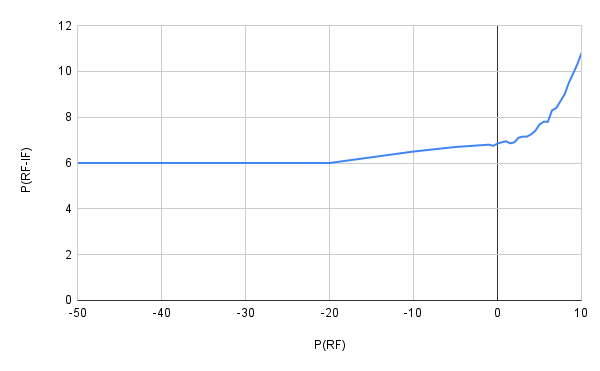
\includegraphics[width=10cm]{ptCompression.png}	
		\caption{Pertes de convertions en fonction de $P_{RF}$}
	\end{figure}

	Le point de compression correspond au point tel que les pertes de convertion se dégradent de 1dB. 
	Ici on voit sur le graph que ce point se trouve autour de $P_{RF}=0dBm$. Avant ce point, les pertes sont constantes autour de 6dB.

	\begin{figure}[h]
		\centering
		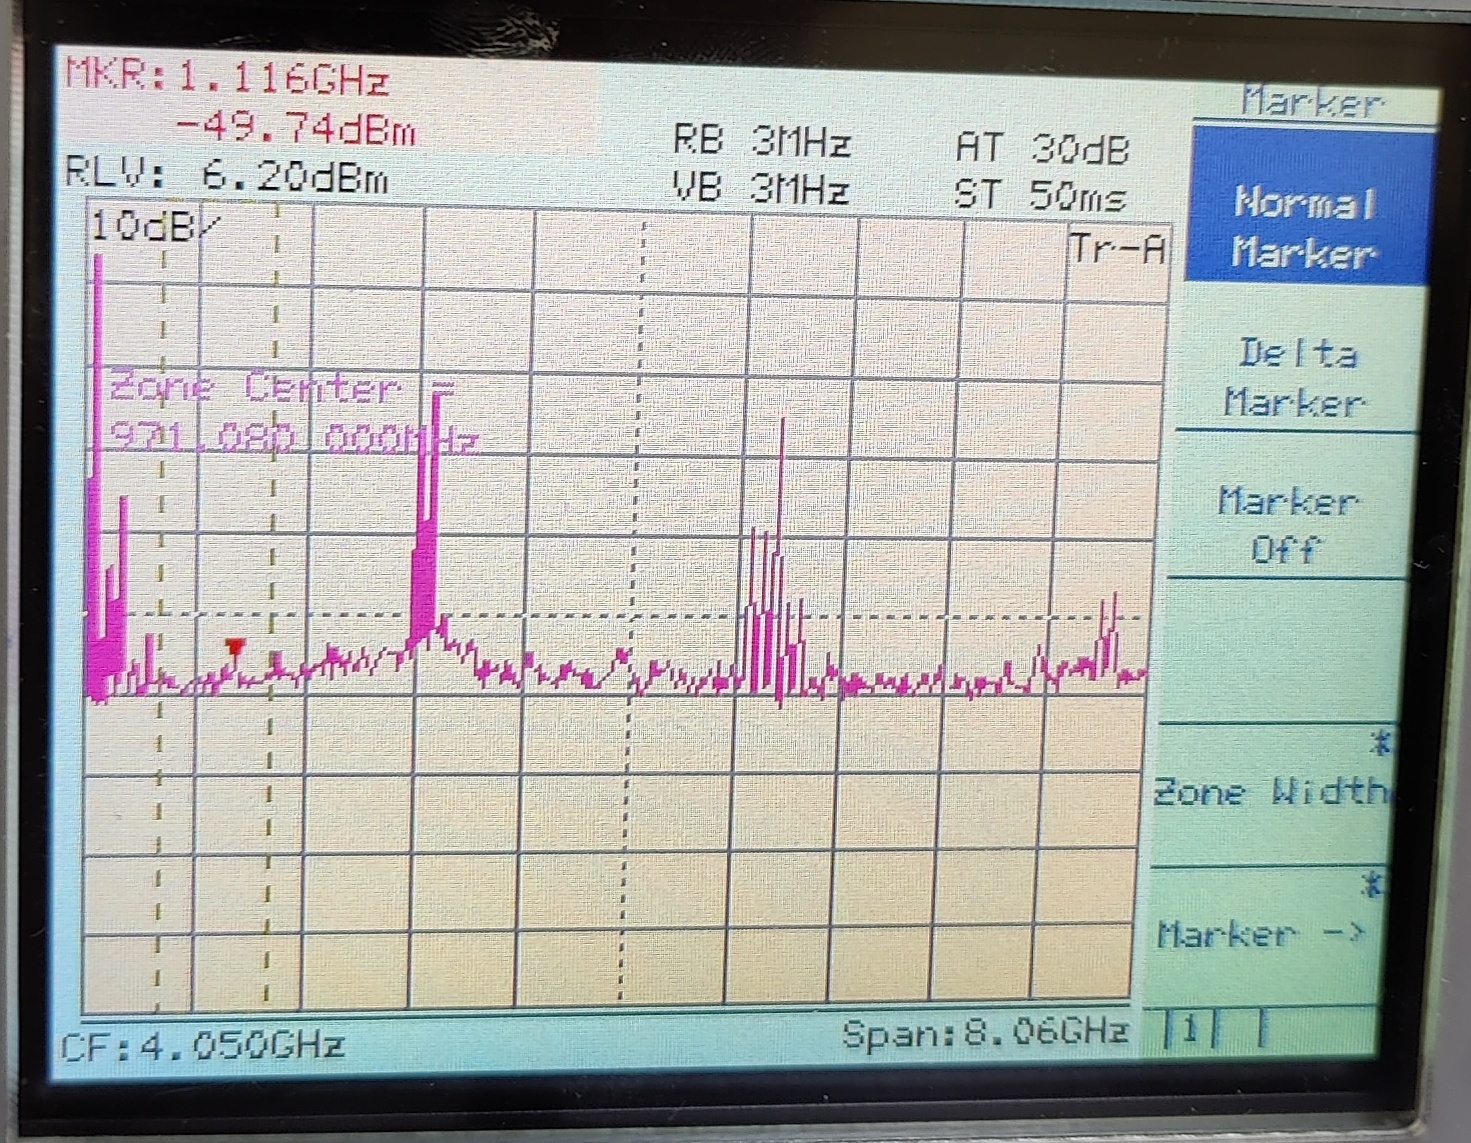
\includegraphics[width=9cm]{manip4.jpg}	
		\caption{Spectre complet en voie IF à $P_{RF} = 10dBm$}
	\end{figure}

	\newpage
	\section{Conclusion}

	Nous avons caractèrisé notre mélangeur par ses pertes et nous avons pu obtenir des graphs qui corroborent ceux de la datasheet.
	On a pu voir que la caractèrisation complète ne nécessite pas beaucoup de matériel (si on omet l'analyseur de spèctre qui n'est pas tout à fait un équipement commun).
	

\end{document}
